% Options for packages loaded elsewhere
\PassOptionsToPackage{unicode}{hyperref}
\PassOptionsToPackage{hyphens}{url}
\PassOptionsToPackage{dvipsnames,svgnames,x11names}{xcolor}
%
\documentclass[
  11pt,
  a4paper,
  krantz2,
  11pt,
  oneside]{krantz}
\usepackage{amsmath,amssymb}
\usepackage{iftex}
\ifPDFTeX
  \usepackage[T1]{fontenc}
  \usepackage[utf8]{inputenc}
  \usepackage{textcomp} % provide euro and other symbols
\else % if luatex or xetex
  \usepackage{unicode-math} % this also loads fontspec
  \defaultfontfeatures{Scale=MatchLowercase}
  \defaultfontfeatures[\rmfamily]{Ligatures=TeX,Scale=1}
\fi
\usepackage{lmodern}
\ifPDFTeX\else
  % xetex/luatex font selection
  \setmainfont[]{Alegreya}
\fi
% Use upquote if available, for straight quotes in verbatim environments
\IfFileExists{upquote.sty}{\usepackage{upquote}}{}
\IfFileExists{microtype.sty}{% use microtype if available
  \usepackage[]{microtype}
  \UseMicrotypeSet[protrusion]{basicmath} % disable protrusion for tt fonts
}{}
\makeatletter
\@ifundefined{KOMAClassName}{% if non-KOMA class
  \IfFileExists{parskip.sty}{%
    \usepackage{parskip}
  }{% else
    \setlength{\parindent}{0pt}
    \setlength{\parskip}{6pt plus 2pt minus 1pt}}
}{% if KOMA class
  \KOMAoptions{parskip=half}}
\makeatother
\usepackage{xcolor}
\usepackage{longtable,booktabs,array}
\usepackage{calc} % for calculating minipage widths
% Correct order of tables after \paragraph or \subparagraph
\usepackage{etoolbox}
\makeatletter
\patchcmd\longtable{\par}{\if@noskipsec\mbox{}\fi\par}{}{}
\makeatother
% Allow footnotes in longtable head/foot
\IfFileExists{footnotehyper.sty}{\usepackage{footnotehyper}}{\usepackage{footnote}}
\makesavenoteenv{longtable}
\usepackage{graphicx}
\makeatletter
\def\maxwidth{\ifdim\Gin@nat@width>\linewidth\linewidth\else\Gin@nat@width\fi}
\def\maxheight{\ifdim\Gin@nat@height>\textheight\textheight\else\Gin@nat@height\fi}
\makeatother
% Scale images if necessary, so that they will not overflow the page
% margins by default, and it is still possible to overwrite the defaults
% using explicit options in \includegraphics[width, height, ...]{}
\setkeys{Gin}{width=\maxwidth,height=\maxheight,keepaspectratio}
% Set default figure placement to htbp
\makeatletter
\def\fps@figure{htbp}
\makeatother
\setlength{\emergencystretch}{3em} % prevent overfull lines
\providecommand{\tightlist}{%
  \setlength{\itemsep}{0pt}\setlength{\parskip}{0pt}}
\setcounter{secnumdepth}{5}
\usepackage{booktabs}
\usepackage{longtable}
\usepackage[bf,singlelinecheck=off]{caption}

\usepackage{framed,color}
\definecolor{shadecolor}{RGB}{248,248,248}

\renewcommand{\textfraction}{0.05}
\renewcommand{\topfraction}{0.8}
\renewcommand{\bottomfraction}{0.8}
\renewcommand{\floatpagefraction}{0.75}

\renewenvironment{quote}{\begin{VF}}{\end{VF}}
\let\oldhref\href
\renewcommand{\href}[2]{#2\footnote{\url{#1}}}

\ifxetex
  \usepackage{letltxmacro}
  \setlength{\XeTeXLinkMargin}{1pt}
  \LetLtxMacro\SavedIncludeGraphics\includegraphics
  \def\includegraphics#1#{% #1 catches optional stuff (star/opt. arg.)
    \IncludeGraphicsAux{#1}%
  }%
  \newcommand*{\IncludeGraphicsAux}[2]{%
    \XeTeXLinkBox{%
      \SavedIncludeGraphics#1{#2}%
    }%
  }%
\fi

\makeatletter
\newenvironment{kframe}{%
\medskip{}
\setlength{\fboxsep}{.8em}
 \def\at@end@of@kframe{}%
 \ifinner\ifhmode%
  \def\at@end@of@kframe{\end{minipage}}%
  \begin{minipage}{\columnwidth}%
 \fi\fi%
 \def\FrameCommand##1{\hskip\@totalleftmargin \hskip-\fboxsep
 \colorbox{shadecolor}{##1}\hskip-\fboxsep
     % There is no \\@totalrightmargin, so:
     \hskip-\linewidth \hskip-\@totalleftmargin \hskip\columnwidth}%
 \MakeFramed {\advance\hsize-\width
   \@totalleftmargin\z@ \linewidth\hsize
   \@setminipage}}%
 {\par\unskip\endMakeFramed%
 \at@end@of@kframe}
\makeatother

\renewenvironment{Shaded}{\begin{kframe}}{\end{kframe}}

\usepackage{makeidx}
\makeindex

\urlstyle{tt}

\usepackage{amsthm}
\makeatletter
\def\thm@space@setup{%
  \thm@preskip=8pt plus 2pt minus 4pt
  \thm@postskip=\thm@preskip
}
\makeatother

\frontmatter
\ifLuaTeX
  \usepackage{selnolig}  % disable illegal ligatures
\fi
\usepackage[]{natbib}
\bibliographystyle{apalike}
\usepackage{bookmark}
\IfFileExists{xurl.sty}{\usepackage{xurl}}{} % add URL line breaks if available
\urlstyle{same}
\hypersetup{
  pdftitle={Automatisation des processus de sécurité},
  pdfauthor={Germain Jr.~OLEA-OYOUGOU},
  colorlinks=true,
  linkcolor={Maroon},
  filecolor={Maroon},
  citecolor={Blue},
  urlcolor={Blue},
  pdfcreator={LaTeX via pandoc}}

\title{Automatisation des processus de sécurité\thanks{Thank you}}
\author{Germain Jr.~OLEA-OYOUGOU}
\date{15 septembre 2024}

\begin{document}
\maketitle

\thispagestyle{empty}
\begin{center}
\Large{Note Personnelle}

\large{Une magnifique citation qui explique l'objectif et le sens profond de ce mémoire}
%\includegraphics{images/dedication.pdf}
\end{center}

\setlength{\abovedisplayskip}{-5pt}
\setlength{\abovedisplayshortskip}{-5pt}

{
\hypersetup{linkcolor=}
\setcounter{tocdepth}{2}
\tableofcontents
}
\listoffigures
\listoftables
\chapter{Résumé}\label{ruxe9sumuxe9}

La question de l'automatisation des processus de sécurité naît du constat de l'incapacité des équipes de sécurité à suivre l'évolution des méthodologies de gestion de projets qui nous emmènent à livrer de plus en plus rapidement nos produits et se retrouvent avec une charge de travail qui aurait pu être amoindri en amont. Cette thèse professionnelle traitera des différents processus de sécurité dans les phases de prévention de détection et de réponse et des possibilités d'automatisation de ces derniers.

En partant de l'origine des besoins de la sécurité de l'information elle donnera des détails sur pourquoi et comment automatiser un processus. Sur la base des travaux de docteurs en sécurité informatique et les rapports de diverses conférences parlant d'automatisation, elle montrera les recommandations de l'industrie en ce qui concerne la mise en place de processus automatisés au sein d'une organisation.

Elle argumente sur l'avantage du Shift Left et des pratiques DevSecOps en donnant des pistes de solutions sur l'adoption d'une approche automatisée de la sécurité dans le contexte de Shadow et en avertissant sur les risques de trop se fier à un système totalement automatisé.

\chapter{Glossaire}\label{glossaire}

\textbf{Shift-Left} : Intégrer les tests et la sécurité dès les premières phases du développement pour détecter les problèmes plus tôt.

\textbf{DevOps} : Méthode combinant développement et opérations pour livrer des logiciels plus rapidement et de manière fiable.

\textbf{DevSecOps} : Extension de DevOps intégrant la sécurité dès le début du cycle de développement.

\textbf{NTA} : Analyse du trafic réseau pour détecter des comportements suspects ou des menaces.

\textbf{IDS/IPS} : Systèmes qui détectent (IDS) et préviennent (IPS) les intrusions ou activités malveillantes.

\textbf{EDR/XDR} : Solutions de sécurité pour détecter et répondre aux menaces sur les terminaux (EDR) ou à travers plusieurs couches (XDR).

\textbf{Delivery first} : Approche visant à livrer rapidement des fonctionnalités ou produits fonctionnels.

\textbf{CI/CD} : Automatisation des tests (CI) et du déploiement (CD) dans le développement logiciel.

\textbf{Linting} : Analyse du code pour détecter des erreurs ou des violations des conventions de codage.

\textbf{Packaging} : Compilation du code en un package ou une unité exécutable pour déploiement.

\textbf{Build} : Compilation du code en une application exécutable, incluant tests et gestion des dépendances.

\chapter{Déclaration sur l'honneur}\label{duxe9claration-sur-lhonneur}

Je déclare sur l'honneur que cette thèse professionnelle est le fruit d'un travail personnel et que je n'ai ni contrefait, ni falsifié, ni copié tout ou partie de l'œuvre d'autrui afin de la faire passer pour mienne.

Toutes les sources d'information utilisées (supports papiers, audiovisuels et numériques) et les citations d'auteur ont été mentionnées conformément aux usages en vigueur.

Je suis conscient que le fait de ne pas citer une source ou de ne pas la citer clairement et complètement est constitutif de plagiat, que le plagiat est considéré comme une faute grave au sein de l'Université de Technologie de Troyes (UTT) et qu'il peut être sévèrement sanctionné.

Je confirme que les propos écrits n'engagent que moi et en aucune façon ni l'UTT ni toute autre partie prenante.

\chapter{Introduction}\label{introduction}

Mes deux ans d\textquotesingle alternance au sein de la société Shadow m\textquotesingle ont montré à quel point elle déploie des efforts pour optimiser son processus de déploiement. Shadow possède deux produits : Shadow PC, un ordinateur à hautes performances dans le Cloud accessible depuis n'importe quel périphérique et Shadow Drive, le stockage en ligne souverain. La gestion de ces deux produits nécessite le développement de plusieurs outils internes, avec cela un nombre de processus de maintenance assez élevés. Pour garder un niveau de qualité élevé et une rapidité dans ces processus, Shadow a misé sur l\textquotesingle automatisation du déploiement de nombreux de ses services avec la mise en place de pratiques DevOps assez avancées. Au sein de l\textquotesingle équipe sécurité nous avons senti le besoin de s\textquotesingle adapter à cette évolution en procédant à un Shift Left, c'est-à-dire insérer les tests de sécurité au plus tôt au sein du cycle de développement pour trouver et corriger les vulnérabilités le plus tôt possible. En opposé au Shift Right qui consiste à exécuter des tests, surveiller le comportement de l'utilisateur et les paramètres de sécurité quand le produit est déjà opérationnel.

La plupart des décisions de sécurité sont prises lors des processus de développement et de mise en condition opérationnelle par ces équipes et les équipes de sécurité ne prennent que très rarement des décisions qui impliquent directement le produit mais plutôt quand il s'agit d'évaluer ou atténuer un risque. Il est difficile de se prémunir de catastrophes commerciales et métier en appliquant des mesures avant la définition des stratégies de sécurité. Pourtant ce mode de fonctionnement est encore courant et ralentit la vélocité des équipes de développement.

Pour éviter de découvrir des vulnérabilités trop tard et de ne réagir qu'en cas d'incident, il est intéressant de se demander comment la mise en place des pratiques de sécurité automatisées au sein des processus de développement peut améliorer la résistance des systèmes d\textquotesingle information aux menaces qui pèsent sur une organisation et augmenter la performance des équipes de sécurité. En tant qu'apprenti chez Shadow j'ai eu le rôle de mener une analyse comparative et de mettre en place ces pratiques afin d'évaluer l'apport en productivité de l'amélioration de nos processus.

Notre objectif à présent est de confronter les visions communes et acceptées par l'industrie sur ce sujet en apportant des pistes d'amélioration et en ajoutant de la valeur sur les défauts apparents. De ce fait pour développer la réponse à cette problématique nous allons étudier l'état de l'art en matière d'automatisation des processus de sécurité et les bénéfices que cela peut apporter tout en analysant les méthodologies de mise en place des pratiques et les outils à intégrer. En parallèle nous discuterons de l'implémentation de ces mesures au sein de Shadow, nous créerons un environnement propice à la pratique des compétences nécessaires à la mise en place de ces méthodologies. Enfin nous ne manquerons pas de lister les limites de ces pratiques et d'aborder les sujets allant au-delà de cette problématique. Toutefois nous ne saurons commencer sans relater le contexte de la sécurité de l'information et les raisons derrière l'automatisation des processus qui font ce domaine.

\chapter{Etat de l\textquotesingle art de l\textquotesingle automatisation des processus de sécurité}\label{etat-de-lart-de-lautomatisation-des-processus-de-suxe9curituxe9}

\section{Contexte sur l'automatisation des processus de sécurité}\label{contexte-sur-lautomatisation-des-processus-de-suxe9curituxe9}

\subsection{La sécurité informatique}\label{la-suxe9curituxe9-informatique}

Pour contextualiser notre sujet, revenons aux origines et définissons la sécurité informatique.

L\textquotesingle objectif de l\textquotesingle informatique est la gestion automatique de l\textquotesingle information et la sécurité informatique implique la sécurité de l\textquotesingle information c\textquotesingle est-à-dire le maintien de la confidentialité, intégrité et la disponibilité de ces informations. Ces trois points sont les piliers de la sécurité informatique. Le principe de confidentialité stipule que l'information ne doit être accessible qu'aux personnes autorisées, l'intégrité est la garantie que l'information ne soit pas corrompue, dégradée ou modifiée et la disponibilité est l'assurance que l'information soit accessible aux personnes autorisées au moment où elles en ont besoin.

La sécurité de l'information n'est pas figée, elle est plutôt le résultat d'un processus d'amélioration continue, c'est-à-dire qui évolue à travers différentes phases et se perfectionne tout le long. Il s'agit d'un voyage et pas une destination. Bien qu'il y ait de nombreuses étapes dans ce voyage nous pouvons néanmoins les regrouper dans trois grandes phases : la prévention, la détection et la réponse (incluant la remédiation) (LaPiedra, 2002).

\subsubsection{La prévention}\label{la-pruxe9vention}

La prévention consiste à se préparer en amont pour se prévenir de futurs incidents. Notre objectif est de protéger l'information de toutes dégradations, altération ou accès non autorisé. Pour cela la phase de prévention implique :

\begin{itemize}
\item
  La définition de politiques de sécurité : savoir ce qui doit être protégé en décrivant des règles claires, concises et précises.
\item
  La mise en place d'un programme de sensibilisation à la sécurité de l'information pour éduquer toute l'équipe aux bonnes pratiques de sécurité et aux risques que court l'organisation
\item
  L'implémentation des contrôles d'accès : restreindre l'accès et n'autoriser que les permissions nécessaires à la fonction de l'utilisateur. Identifier correctement les principes d'identification, authentification et autorisation dans chaque processus d'accès.
\end{itemize}

\subsubsection{La détection}\label{la-duxe9tection}

Se protéger est idéal mais détecter est indispensable. Tout système d'information est vulnérable et sujet à compromission. Keith Alexander, général de la United States Army et directeur de la National Security Agency (NSA) affirme durant la U.S. Chamber of Commerce Cybersecurity Summit en 2012 :

\begin{quote}
Either you know you've been hacked, or you've been hacked and you don't know you've been hacked
\end{quote}

que nous pouvons traduire par : soit vous savez que vous avez été attaqué soit vous avez été attaqué mais vous ne le savez pas encore. En effet, peu importe le niveau de protection d'un système d'information, ce n'est qu'une question de temps avant qu'il ne soit compromis par un acteur ayant assez de compétences et de motivation. D'où l'importance d'un système de détection de d'intrusion et de compromission (IDS). Le facteur le plus crucial dans une stratégie de détection est le temps moyen entre l\textquotesingle infection et la détection ajoutée à la précision de la notification en cas de compromission : une détection plus rapide et une notification plus précise amélioreront l\textquotesingle efficacité du processus d\textquotesingle investigation et de réponse en cas d\textquotesingle incident.

\subsubsection{La réponse}\label{la-ruxe9ponse}

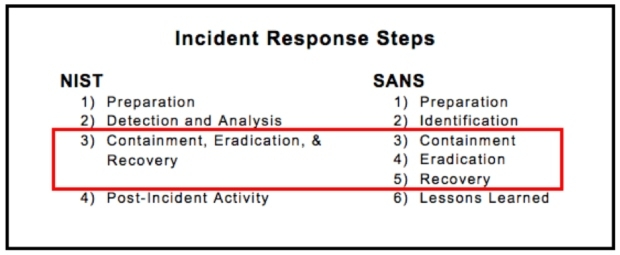
\includegraphics{./assets/img/sans-nist-ir-annotated.jpeg}

La réponse consiste à réagir face à l'annonce d'un nouvel incident ou d'une compromission. La phase de réponse donne toute sa valeur à une détection de qualité. Néanmoins, une bonne réponse ne s'improvise pas. Le stress que nous ressentons lors d'une attaque ne permet pas de prendre de bonnes décisions. Il existe des méthodologies de réponse à incident permettant d'adapter son plan de réponse à son métier et à l'incident subit. Celui du NIST (National Institute of Standards and Technology) et du SANS se distingue dans le schéma suivant.

Nous commençons toujours par l'étape de préparation qui se déroule en général avant l'arrivée de l'incident. La détection arrive ensuite, nous devons identifier et analyser le type d'attaque que nous subissons, son origine et idéalement l'auteur de l'attaque. Après cela le confinement vise à réduire l'impact de l'incident, l'éradication à supprimer la menace du système d'information et la reprise à remettre le système en condition opérationnelle. Enfin la dernière étape consiste toujours à faire une revue de la gestion de l'incident et sert à améliorer le processus de réponse en lui-même.

Une bonne réponse à incident nécessite un processus rapide qui aboutit à une remédiation dans un court laps de temps. Au-delà d'une succession optimale des étapes susmentionnées, nous devons noter que la vitesse de ce processus passe par une remontée efficace des informations nécessaire à l'équipe lors de la détection même l'incident. Le SANS précise que

\begin{quote}
The process of detecting malicious or accidental misuse of resources is much more than sounding an alarm. Also, responding to an incident is much more than just showing up. An organization to be successful must know what to detect and once alerted know how to effectively coordinate resources for a response.
\end{quote}

Pour poursuivre, une bonne détection est de même liée à une préparation et une prévention correcte. Là se trouvent les principaux maux de la sécurité informatique :

\begin{itemize}
\item
  Ils prennent du temps
\item
  Ils nécessitent beaucoup de bande passante (de charge de travail, de personnes qualifiées)
\item
  Ils sont coûteux en ressources et en argent
\end{itemize}

Cela décourage certaines organisations à entamer le voyage dont nous parlons. Comment donc faire en sorte de corriger ces barrières tout en facilitant l'adoption des pratiques de sécurité ? Chez Shadow nous avons un programme de sécurité établi par Florent notre responsable sécurité. Après avoir fait l'état des lieux et défini les politiques nécessaires et les actions à prendre pour commencer notre voyage, ce dernier inclut une phase d'automatisation des processus de sécurité au sein du cycle de développement mais également dans les tâches quotidiennes de l'équipe en charge de la sécurité.

\subsection{Les processus de sécurité automatisées}\label{les-processus-de-suxe9curituxe9-automatisuxe9es}

Dans un monde idéal, nous n\textquotesingle aurions pas à répondre à des incidents ou, du moins, nous n\textquotesingle aurions qu\textquotesingle à traiter des incidents dignes de notre attention. L\textquotesingle une des solutions pour parvenir à ce monde idéal serait d\textquotesingle automatiser les processus répétitifs.

Le docteur Brian Carrier définit l'automatisation en disant :

\begin{quote}
Automation is when the computer does the next step without human intervention\footnote{Mentionné dans la conférence : \href{https://www.youtube.com/watch?v=P1ghXLKb_1Y}{To Automate or Not to Automate : That is the Incident Response Question}}
\end{quote}

De ce fait l'automatisation des processus de sécurité permettrait~:

\begin{itemize}
\item
  Une réduction des tâches manuelles de bas niveau : pour libérer du temps à l\textquotesingle équipe sécurité et lui permettre de se concentrer sur les tâches nécessitant plus d\textquotesingle attention.
\item
  Une réponse rapide aux incidents : pour réduire le MTTD (Mean Time To Detect --- temps moyen de détection) et le MTTR (Mean Time To Repair --- temps moyen de réparation) comme expliqué plus haut.
\item
  Une standardisation des processus : car une plateforme automatisée suivra toujours les règles que nous lui donnons, éliminant ainsi les erreurs d\textquotesingle opérations manuelles et apportant de la cohérence.
\item
  Un gain de productivité général pour l\textquotesingle équipe.
\end{itemize}

Cependant, l\textquotesingle automatisation n\textquotesingle est pas l\textquotesingle unique option. Les autres solutions consistent à optimiser la réalisation des processus en améliorant ceux qui en dépendent. Par exemple, nous pouvons limiter le temps de réponse à un incident en maximisant les indicateurs que nous remontent nos systèmes de détection d\textquotesingle intrusion (IDS). Nous pouvons également élever le niveau de notre détection en connaissant profondément notre système d\textquotesingle information. En effet, une connaissance parfaite de son SI et de ses services permet de configurer finement ses outils de détection et de remonter les événements. En continuant avec cette idée, on éviterait le nombre d\textquotesingle événements remontés en prévenant le nombre de vulnérabilités dans nos applications, réduisant ainsi notre surface d\textquotesingle attaque et, par transitivité, le risque auquel nous sommes soumis. D\textquotesingle où l\textquotesingle importance de la phase de prévention.

Une grosse partie de la prévention est de faire en sorte que les applications et logiciels que nous sortons soient sécurisés, nous arrivons donc à la sécurisation du cycle de développement.

\subsection{Le cycle de développement sécurisé}\label{le-cycle-de-duxe9veloppement-suxe9curisuxe9}

Tenant ses origines des années 1960, la sécurité dans le SDLC --- Software Development Lifecycle --- et toutes les méthodologies s'en inspirant, quand elle est incluse, se positionne comme un jalon la gestion de projet entre certaines étapes du SDLC. Une porte à franchir pour passer à l'étape suivante. Nous avons généralement dans les équipes soucieuses de la sécurité de leur produit

\begin{itemize}
\item
  La revue des spécifications et de la conception du produit : après l'étape d'identification
\item
  La revue de l'architecture : après l'étape de conception
\item
  La revue du code : après l'étape de création ou développement
\item
  Les tests de sécurité : après l'étape des tests.
\end{itemize}

Laura Bell précise dans son livre \emph{Agile Application Security} que l'idée derrière ces jalons soit de réaliser des livrables en lot car

\begin{quote}
It is predicated on the old rule that the earlier a defect is caught, the cheaper it is to fix; therefore we need to do a security review as early as possible to catch security defects before they get too far. (Bell, Brunton-Spall, Smith, \& Bird, 2017, p.~79)
\end{quote}

Sauf que notre problématique persiste. Effectivement, les processus et pratiques de sécurité telles que nous les connaissons ont été conçues pour une gestion de projet en cascade où les besoins sont décidés bien avant et pas pour des petites équipes évoluant rapidement et de manière itérative.

En optant pour une approche Agile, la solution ne consisterait pas à résoudre tous les problèmes de sécurité avant la mise en production, mais plutôt à se concentrer sur la réduction du coût de correction, en rendant les futurs changements sans risque et plus facilement réalisables.

\begin{quote}
We want to reach a fine balance between finding and fixing (or better, preventing) security problems up front where it makes sense to do so, and making sure that we can fix them quickly and cheaply later if something gets by. (Bell, Brunton-Spall, Smith, \& Bird, 2017, p.~79)
\end{quote}

La première approche pour répondre à cela est l'apparition du principe \emph{Shift Left}\footnote{L'article de RedHat \href{https://www.redhat.com/en/topics/devops/shift-left-vs-shift-right}{\emph{Shift-Left vs Shift-Right}} aborde en profondeur ce sujet.}\emph{,} c'est-à-dire inclure des tests de sécurité à chaque étape du SDLC. Nous obtenons ce dont les experts appellent le SSDLC --- Secure Development Lifecycle --- ou SDL pour faire court. (Voir annexe 1)

Une approche plus récente avec la montée en charge des pratiques DevOps et l'augmentation exponentielle des menaces de sécurité, permet d'aller encore plus loin et favorise les entreprises à se préparer et à actualiser fréquemment l'ensemble de ses processus de sécurité de la prévention à la réponse : le modèle DevSecOps avec un accent particulier sur l'automatisation.

Dans le parcours de la sécurité chez Shadow, j'ai eu l'honneur d'avoir la responsabilité de mettre en place certaines de ces pratiques. Cependant, maintenant que nous savons pourquoi l'automatisation peut être un acteur positif à l'évolution des processus de sécurité, découvrons ce qui se fait de mieux avant d'aborder concrètement les actions menées au sein de notre organisation.

\section{Introduction à l'automatisation}\label{introduction-uxe0-lautomatisation}

Avant de parler d'automatisation et de pratiques DevSecOps, nous devons savoir \emph{Quoi} automatiser et \emph{Quand} automatiser. Mentionné plus tôt, le Dr.~Brian Carrier défini trois niveaux d'automatisation pour compléter sa définition

\begin{enumerate}
\def\labelenumi{\arabic{enumi}.}
\item
  Manuelle : c'est-à-dire aucune présence de quelconque automatisation.
\item
  Partielle : une automatisation présente mais ayant besoin de quelques interactions humaines.
\item
  Totale : définissant un processus totalement automatisé.
\end{enumerate}

Quand nous souhaitons automatiser, nous devons choisir le niveau d\textquotesingle automatisation selon que :

\begin{itemize}
\item
  le \textbf{bénéfice} qu'apportera la réalisation automatique de la prochaine étape du processus soit assez élevé
\item
  le \textbf{coût} humain, logiciel et matériel de la mise en place du processus automatique soit abordable dans notre contexte
\item
  la \textbf{probabilité} qu'une erreur survienne et son \textbf{impact} extérieur à son contexte soit acceptable
\end{itemize}

Sachant que plus une automatisation devient complexe, plus le besoin en ressources matérielles et en maintenance se fait grand, nous devons évaluer ces paramètres non seulement au début de la phase de réflexion de la mise en place de notre processus automatisé mais aussi à chaque fois que nous souhaitons faire évoluer notre niveau d'automatisation.

En ce qui concerne le cycle de développement notre objectif en faisant du \emph{Shift Left} est d'accompagner le développeur et de lui faire un retour \emph{continu} sur son code. Voyant ce que nous apporte le DevSecOps sur ce chemin.

\section{Prévention et DevSecOps}\label{pruxe9vention-et-devsecops}

Plus qu'une recette miracle ou un terme new age, le DevSecOps est une approche et une philosophie qui comme les principes Agiles favorise la collaboration entre les équipes dans l'objectif de détecter au plus tôt les problèmes de sécurité et les vulnérabilités diverses. L'OWASP dit dans le projet \textbf{OWASP DevSecOps Guideline}

\begin{quote}
The Ideal goal is ``detect security issues (by design or application vulnerability) as fast as possible.''\footnote{\href{https://owasp.org/www-project-devsecops-guideline/}{OWASP DevSecOps Guideline}}
\end{quote}

On peut voir le DevSecOps comme une aide et un ensemble de bonnes pratiques dans la mise en place d'un cycle de développement sécurisé.

\subsection{Culture DevSecOps}\label{culture-devsecops}

Le terme DevSecOps suppose l'engagement des équipes développement, sécurité et opérationnelle. Sauf que cette approche va au-delà de la définition même de ces équipes et implique tous les métiers agissant sur le cycle de développement pour les rendre responsables de la sécurité : du chef de projet aux développeurs en passant par les designers, les architectes, etc. De plus Shannon Lietz --- fondateur de la DevSecOps Foundation dit

\begin{quote}
The purpose and intent of DevSecOps is to build on the mindset that ``everyone is responsible for security'' with the goal of safely distributing security decisions at speed and scale to those who hold the highest level of context without sacrificing the safety required.''\footnote{\href{https://www.devsecops.org/blog/2015/2/15/what-is-devsecops}{What is DevSecOps}}
\end{quote}

Pour cela, nous devons sensibiliser nos équipes à la culture DevSecOps et mettre en place des outils pour parvenir à une stratégie de Shift Left performante. L\textquotesingle étape préalable consiste à comprendre l\textquotesingle importance d\textquotesingle un esprit de collaboration, ce qui constitue une base solide pour le partage des bonnes pratiques de sécurité au sein des équipes. Cela facilite également le travail des équipes de sécurité dans la compréhension de leurs politiques par les collaborateurs. D'où la nécessité d'un programme de sensibilisation à la sécurité informatique. Notamment la compréhension des vulnérabilités venant des standards comme le OWASP Top 10 ou le CWE top 25.

\subsection{Comprendre son besoin en sécurité}\label{comprendre-son-besoin-en-suxe9curituxe9}

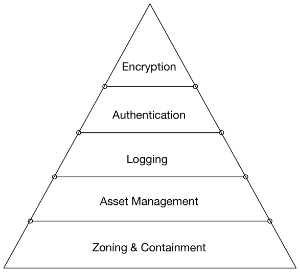
\includegraphics{./assets/img/Hierarchy of software security needs.png}

Avant de se lancer dans un programme de mise en place de pratiques DevSecOps une organisation doit prendre en compte son niveau de maturité pour pouvoir formaliser son besoin de sécurité et pouvoir le traduire en tant que processus automatisé. Un article de Shannon Lietz présente une pyramide pour hiérarchiser les besoins en sécurité d'un logiciel à la manière de la pyramide de Maslow.\footnote{\href{https://www.devsecops.org/blog/2016/5/20/-security}{Shifting Security to the Left}}

Hiérarchiser ses besoins permet de mieux répartir nos efforts dans la mise en place de politique de sécurité. Nous l'avons dit, la sécurité informatique n'est pas figée, ainsi nos politiques doivent être faites selon la culture, les objectifs et les politiques organisationnelles de l'entreprise. De la même manière notre approche vers l'automatisation de nos processus de sécurité ne doit pas être figée à un unique standard. Nous devons prendre en compte les contraintes de chaque outil avant de faire notre choix, s'assurer que toute l'équipe adopte un schéma de pensé aligné avec l'idée de ne pas faire de choix qui sembleraient couvrir tous les besoins existant mais plutôt s'orienter vers des solutions qui répondent à un besoin particulier. Par exemple choisir un outil pour un langage de programmation spécifique quand cela est pertinent plutôt qu'un autre promettant de réaliser un traitement sur tous types de langage mais sans réelle efficacité.

Il existe des outils qui nous aident dans l'évaluation de notre niveau de maturité et nous permettent de savoir comment hiérarchiser nos besoins.

\begin{itemize}
\item
  L'OWASP Software Assurance Maturity Model (SAMM) par exemple est un cadre qui a pour objectif d'accompagner les organisations à formuler et à mettre en place une stratégie de sécurité logicielle parfaitement adaptée aux risques spécifiques auxquels l'organisation est confrontée.
\item
  L'OWASP DevSecOps Maturity Model (DMM) est l'équivalent du SAMM pour les pratiques DevSecOps, ce cadre évalue le niveau de mise en place de pratiques DevSecOps au sein de l'organisation, nous aidant à hiérarchiser nos besoins dans notre approche de sécurisation de notre cycle de développement.
\end{itemize}

\subsection{Conception sécurisé et industrialisation des tests}\label{conception-suxe9curisuxe9-et-industrialisation-des-tests}

Une fois qu'une culture de collaboration est établie et que nous savons où orienter nos efforts, nous devons accompagner l'équipe de développement dans la réalisation de sa tâche tout en l'aidant à livrer une application sécurisée. Laura Bell dit dans Agile Application Security

\begin{quote}
Security teams that try to reduce risk by minimizing change, rather than supporting development teams to realize their ideas in a secure way, are doomed to be increasingly irrelevant in an Agile world, and will therefore be bypassed.

\[...\] Security professionals have to learn to accept change, to work faster and more iteratively, and be able to think about security risks, and how to manage risks, in incremental terms. And most important\textbf{, security needs to become an enabler, instead of a blocker.} (Bell, Brunton-Spall, Smith, \& Bird, 2017, p.~76)
\end{quote}

Dans cette direction, qui s'aligne avec le fait de prévenir la découverte de vulnérabilités au plus tôt, notre rôle revient à se retrouver dans le quotidien de l'équipe de développement et au sein de ses outils. Cela se traduit notamment dans la mise en place

\begin{itemize}
\item
  de revue de code sécurisé
\item
  d'un programme de Security Champion, qui est collaborateur de l'équipe ayant un rôle de développeur ou d'opérationnelle en charge de partager une culture de sécurité et de s'assurer du respect des politiques de sécurité lors des développements.
\item
  de tests de sécurité directement dans les cycles d'intégration et de déploiement continu (CI/CD)
\end{itemize}

Le modèle OWASP d'un cycle de livraison continu adapté aux tests de sécurité se présente grossièrement comme suite

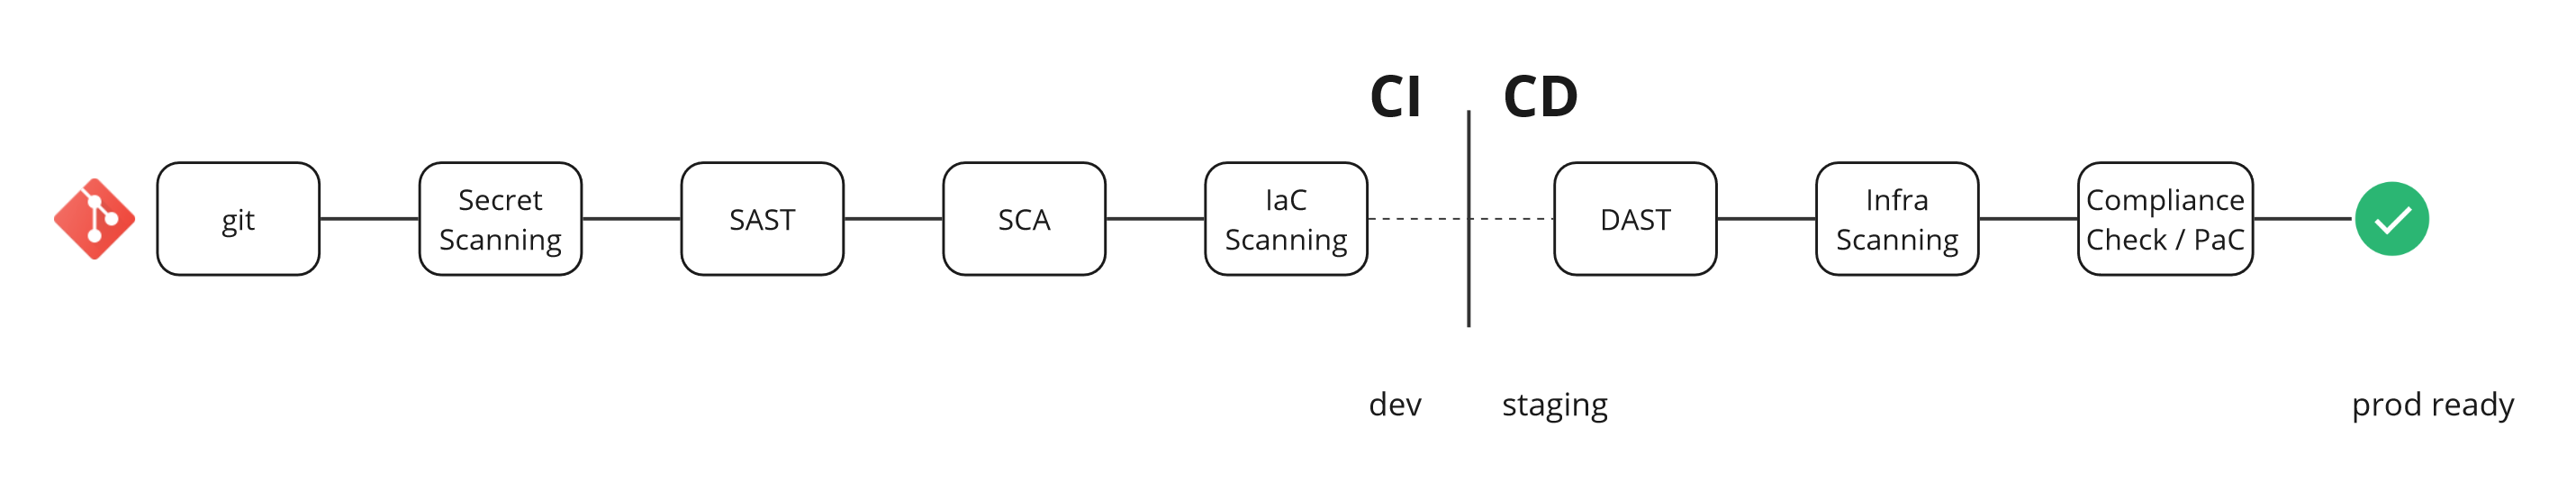
\includegraphics{./assets/img/ci_cd.png}

Ces étapes consistent concrètement à :

\begin{enumerate}
\def\labelenumi{\arabic{enumi}.}
\item
  Parcourir les dépôts git à la recherche d\textquotesingle identifiants ou de valeurs secrètes exposés publiquement.
\item
  Analyser le code source de l\textquotesingle application ou du logiciel à déployer pour découvrir de potentielles vulnérabilités (Static Application Security Testing --- SAST).
\item
  Analyser l\textquotesingle ensemble des composants et librairies dont dépend le code source pour se prémunir des risques de sécurité liés à la compromission de ces derniers (Software Component Analysis --- SCA).
\item
  Réaliser des tests de sécurité sur l\textquotesingle application pendant qu\textquotesingle elle s\textquotesingle exécute, similaire à une activité de tests de pénétration en boîte noire. L\textquotesingle objectif est de retrouver des failles et des vulnérabilités donnant des accès non autorisés aux données (Dynamic Application Security Testing --- DAST).
\item
  Analyser le code destiné à la création dynamique de l\textquotesingle infrastructure pour éviter les erreurs liées à une mauvaise configuration ou une implémentation inadéquate (Infrastructure as Code Scanning --- IaC).
\item
  Analyser \textbf{l\textquotesingle infrastructure} en elle-même pour vérifier l\textquotesingle exposition et la surface d\textquotesingle attaque de l\textquotesingle environnement.
\item
  Tester l\textquotesingle application des politiques définies et la conformité aux différents standards liés à notre industrie (Compliance Check).
\end{enumerate}

Ces dernières se réalisent bien évidemment de manière automatique pour apporter un retour continu aux développeurs dans la correction des vulnérabilités \textbf{remontées}. Mais l\textquotesingle automatisation ne s\textquotesingle arrête pas là. Nous verrons dans la suite que nous pouvons encore faire évoluer l\textquotesingle automatisation de certains de nos processus, mais également quels outils nous permettront d\textquotesingle implémenter ces actions, notamment dans le contexte de Shadow.

Le guide OWASP DevSecOps Guideline\footnote{\href{https://owasp.org/www-project-devsecops-guideline/}{OWASP DevSecOps Guideline}} détaille chacune de ces étapes et apporte des clés et des outils en \textbf{source} ouverte pour nous aider dans notre démarche.

\subsection{Surveiller continuellement}\label{surveiller-continuellement}

De nos jours, les attaquants ne cessent de renouveler leurs techniques d\textquotesingle attaque en profitant du principe de confiance établi entre les environnements et les composants de notre système d\textquotesingle information et ceux de nos organisations partenaires. Certaines méthodes non conventionnelles prolifèrent, notamment en prenant avantage des services en SaaS et en Cloud, car l\textquotesingle attaquant peut facilement s\textquotesingle y introduire et se servir de la base de confiance que nous avons en ces services pour pénétrer au sein de notre environnement. C\textquotesingle est le principe d\textquotesingle une attaque en \emph{Supply Chain}. Ce genre d\textquotesingle attaque est difficile à reconnaître et donne aux attaquants un bon moyen de contourner les outils de détection mis en place. De plus, nos environnements ne sont pas encore prêts pour les détecter. De la même manière que les méthodes d\textquotesingle attaque évoluent, les techniques de détection doivent évoluer. En effet, de la détection d\textquotesingle intrusion réseau et machine que nous connaissons, nous devons tendre vers une détection proche de la logique de l\textquotesingle application et du logiciel en cours de développement. Shannon Lietz dit :

\begin{quote}
The natural evolution of security is from network to host to software.
\end{quote}

C\textquotesingle est-à-dire étudier et comprendre comment notre produit fonctionne et est utilisé pour faire remonter les comportements déviants. Cela implique un développement qui prend en compte une récolte de données importante et pertinente pour une investigation.

Surveiller continuellement, c\textquotesingle est instrumentaliser l\textquotesingle analyse de ces données pour avoir une vision \textbf{claire} du comportement de notre produit en permanence. Cela nécessite un investissement de temps et d\textquotesingle efforts pour comprendre quels sont ces comportements déviants à l\textquotesingle utilisation normale de notre application dans un premier temps, puis comment implémenter les logiques de détection de ces comportements au sein de nos outils. Par exemple, quand nous avons une application d\textquotesingle administration conçue pour être utilisée entre 8 h et 17 h et qu\textquotesingle un utilisateur se connecte à 00 h, nous devons journaliser cet événement de manière particulière pour permettre aux outils de sécurité de lancer une alerte et déclencher une intervention. Pour aller plus loin dans le processus d\textquotesingle automatisation, dans certains cas, l\textquotesingle application peut être conçue et développée pour s\textquotesingle auto-remédier face à ce type de comportement pré-identifié.

En somme, ces pratiques issues de l\textquotesingle approche DevSecOps nous permettent de \emph{Shift Left}, c\textquotesingle est-à-dire détecter les causes d\textquotesingle un manque de sécurité au plus tôt dans le cycle de développement. Comme dit le manifeste DevSecOps :

\begin{quote}
We will not wait for our organizations to fall victim to mistakes and attackers. We will not settle for finding what is already known; instead, we will look for anomalies yet to be detected.
\end{quote}

En réalisant tout cela dans notre phase de prévention de la menace, nous sommes déjà à l\textquotesingle abri de 99\% des attaques courantes. Toutefois, comme nous l\textquotesingle avons déjà abordé, sans détection efficace, nous restons des cibles faciles pour des techniques d\textquotesingle attaque nouvelle génération. Voyons donc comment, en mettant en avant l\textquotesingle automatisation de nos processus, nous pouvons tendre vers l\textquotesingle optimisation de notre système de détection.

\section{Détection de nouvelles menaces}\label{duxe9tection-de-nouvelles-menaces}

La détection est une phase du cycle de sécurité d\textquotesingle une organisation dont l\textquotesingle objectif est d\textquotesingle identifier les menaces présentes au sein du système d\textquotesingle information ou du réseau de cette dernière. Ces menaces peuvent être présentes sous la forme de logiciels malveillants, d\textquotesingle une première prise de contact comme un phishing ou d\textquotesingle un premier accès au réseau, comme une analyse de ports ouverts. Ce processus devrait également être automatisé pour qu\textquotesingle il soit pleinement utile à l\textquotesingle équipe. En effet, beaucoup d\textquotesingle équipes réalisent encore aujourd\textquotesingle hui des investigations manuelles pour faire de la détection de bas niveau, ce qui est malheureusement sujet à des erreurs humaines et à un risque de non-détection de certaines menaces.

Automatiser la détection de menaces implique d\textquotesingle avoir un bon niveau de surveillance des événements sur les terminaux de notre système informatique. Cela va de pair avec une bonne stratégie de notification et réduction du temps à la détection de la menace. James LaPiedra dit dans un document de la certification GIAC du SANS :

\begin{quote}
defense in layers strategy should be deployed so when each layer fails, it fails safely to a known state and sounds an alarm (LaPiedra, 2002)
\end{quote}

Cela devient encore plus vrai face à la montée croissante de nouvelles sortes d\textquotesingle attaques devenant de plus en plus complexes à identifier. D\textquotesingle un autre côté, les anciennes sont facilement identifiables grâce à leur signature particulière et leur schéma déjà bien connu. Dans ce contexte, nous avons tout à y gagner à faire confiance à des outils qui se chargent de ces tâches à notre place pour que nous puissions nous concentrer sur la levée de suspicions sur une menace ou l\textquotesingle identification de menaces plus critiques.

Beaucoup de solutions existent aujourd\textquotesingle hui pour nous accompagner dans cette phase, chacune à différents niveaux du système d\textquotesingle information.

\subsection{Détection au sein du réseau}\label{duxe9tection-au-sein-du-ruxe9seau}

L\textquotesingle analyse du trafic réseau ou \emph{Network Traffic Analysis} (NTA) est une pratique cruciale dans la sécurité d'un système informatique, visant à surveiller et à analyser le trafic réseau pour détecter les anomalies, les menaces et les comportements malveillants. En combinant diverses technologies, elle permet une détection et une aide à la réponse proactives aux incidents de sécurité.

Nous avons notamment

\subsubsection{Les IDS}\label{les-ids}

Les systèmes de détection d'intrusions (IDS), essentiels pour l\textquotesingle analyse du trafic réseau. Surveille le réseau et identifie les activités suspectes ou malveillantes. Comme Snort, un IDS open source très populaire qui analyse le trafic en temps réel et détecte diverses attaques et intrusions.

Chez Shadow nous avons pu mettre en place CrowdSec une solution de sécurité qui analyse les logs applicatifs pour détecter et prévenir les intrusions. Ne se limitant pas qu'à cette tâche, je la présenterai plus loin dans le contexte de la mise en place de détection de la menace au sein de Shadow.

\subsubsection{La suite Elastic Stack (ELK)}\label{la-suite-elastic-stack-elk}

Elastic Stack, également connu sous le nom de ELK (Elasticsearch, Logstash, Kibana), est une suite d\textquotesingle outils open source pour la gestion et l\textquotesingle analyse des données :

\begin{itemize}
\item
  \textbf{Collecte et ingestion de données (Logstash)} : Agrège et traite les données de diverses sources.
\item
  \textbf{Recherche et analyse (Elasticsearch)} : Fournit des capacités de recherche et d\textquotesingle analyse performantes.
\item
  \textbf{Visualisation des données (Kibana)} : Permet la création de tableaux de bord interactifs pour visualiser et explorer les données de sécurité.
\end{itemize}

Le choix et l\textquotesingle intégration de ces technologies NTA permettent de renforcer la visibilité sur le réseau, d\textquotesingle améliorer la détection des menaces et de réagir rapidement aux incidents de sécurité, contribuant ainsi à une posture de sécurité globale plus robuste et réactive.

\subsection{Détection au sein des terminaux du système informatique}\label{duxe9tection-au-sein-des-terminaux-du-systuxe8me-informatique}

Pour détecter les menaces sur nos terminaux de manière automatique nous avons les technologies de Détection et Réponse sur les Endpoints (Endpoint Detection and Response --- EDR) et Détection et Réponse Étendues (EXtended Detection and Response --- XDR). Elles sont cruciales pour la surveillance et la sécurisation des points d\textquotesingle accès réseau, des serveurs et des postes de travails de nos collaborateurs. Elles permettent de détecter, d\textquotesingle analyser et de répondre aux menaces de manière proactive, assurant une protection renforcée des infrastructures informatiques.

L\textquotesingle EDR se concentre sur la détection et la réponse aux menaces directement sur les endpoints (postes de travail, serveurs, appareils mobiles), utilisant des techniques avancées pour identifier les comportements suspects et les activités malveillantes mais également fournir des fonctionnalités adéquates pour enquêter sur les incidents de sécurité et prendre des mesures correctives.

\begin{itemize}
\tightlist
\item
  OpenEDR par exemple est une solution open source qui offre une visibilité complète sur les activités des endpoints, permettant de détecter et de répondre aux menaces en temps réel. OpenEDR est conçu pour être flexible et extensible, ce qui le rend adapté à une variété d\textquotesingle environnements de sécurité. Non seulement il détecte les menaces, mais il permet également aux administrateurs de comprendre l\textquotesingle ampleur des incidents et de mettre en place des réponses efficaces pour limiter les impacts.
\end{itemize}

L\textquotesingle XDR va au-delà de l\textquotesingle EDR en intégrant des données provenant de plusieurs sources de sécurité pour offrir une visibilité et une protection plus globales. Il combine des données de sécurité provenant des endpoints, des réseaux, des serveurs et des applications pour une vue holistique des menaces. Il permet une analyse centralisée des menaces et une réponse coordonnée à travers l\textquotesingle ensemble de l\textquotesingle infrastructure.

\begin{itemize}
\tightlist
\item
  Nous pouvons citer Wazuh comme plateforme open source qui offre des capacités de détection et de réponse étendues. Wazuh intègre des fonctionnalités de surveillance des fichiers, de gestion des configurations, de détection des anomalies et de réponse aux incidents, couvrant ainsi un large spectre de sources de données de sécurité.
\end{itemize}

L\textquotesingle utilisation de solutions EDR et XDR comme OpenEDR et Wazuh permet aux organisations de renforcer leur posture de sécurité en offrant une visibilité accrue et une capacité de réponse améliorée aux menaces. Ces technologies sont essentielles pour détecter et neutraliser les cyberattaques avant qu\textquotesingle elles ne causent des dommages significatifs. Chez Shadow nous avons fait le choix d'intégrer Wazuh à la gamme de nos outils de détection pour couvrir tous nos serveurs de données et machines virtualisées. Un sujet que nous développerons plus loin dans ce document.

\subsection{Gestion des événements détecter}\label{gestion-des-uxe9vuxe9nements-duxe9tecter}

Bien que ces solutions de détection soient suffisantes ; la gestion des informations et des événements de sécurité ou Security Information and Event Management (SIEM) est une approche et une solution essentielle à avoir en matière de détection, elle combine la gestion des informations de sécurité (SIM) et la gestion des événements de sécurité (SEM). Elle permet une analyse en temps réel des alertes de sécurité, contribuant à la détection, la prévention et la réponse aux menaces et incidents de sécurité, tout en assurant la conformité réglementaire des organisations. Elle implique de récolter un grand nombre d'informations des différentes solutions intégrées et de les centraliser pour pouvoir les traiter proprement et faciliter le travail des analystes.

Voici un aperçu de quelques solutions SIEM majeures et leurs caractéristiques distinctives.

\subsubsection{IBM QRadar}\label{ibm-qradar}

IBM QRadar est une plateforme SIEM de premier plan qui se distingue par :

\begin{itemize}
\item
  \textbf{Détection avancée des menaces} : Utilisation de l\textquotesingle apprentissage automatique et de l\textquotesingle analyse comportementale.
\item
  \textbf{Réponse intégrée aux incidents} : Capacités de réponse rapides et efficaces.
\item
  \textbf{Scalabilité} : Adaptée aux grandes entreprises.
\item
  \textbf{Gestion de la conformité} : Conformité avec des normes telles que le RGPD, HIPAA et PCI-DSS.
\end{itemize}

\subsubsection{SPLUNK}\label{splunk}

Splunk est réputé pour sa gestion des grandes quantités de données générées par les machines. Ses caractéristiques incluent :

\begin{itemize}
\item
  \textbf{Surveillance en temps réel} : Alertes instantanées sur les menaces.
\item
  \textbf{Ingestion de données polyvalente} : Adaptabilité à divers environnements.
\item
  \textbf{Recherche et visualisation performantes} : Capacités de recherche approfondies et visualisations intuitives.
\item
  \textbf{Tableaux de bord personnalisables} : Suivi des indicateurs de performance spécifiques.
\end{itemize}

\subsubsection{Datadog Cloud SIEM}\label{datadog-cloud-siem}

Datadog Cloud SIEM, une solution native du cloud, offre :

\begin{itemize}
\item
  \textbf{Architecture native du cloud} : Déploiement facile et évolutivité.
\item
  \textbf{Surveillance unifiée} : Intégration avec les autres services de Datadog.
\item
  \textbf{Détection automatisée des menaces} : Algorithmes d\textquotesingle apprentissage automatique pour la détection proactive.
\item
  \textbf{Gestion des incidents} : Outils efficaces pour une réponse rapide.
\end{itemize}

Avoir une approche de gestion des événements de sécurité avec une solution SIEM doit prendre en compte la taille de l\textquotesingle organisation, des exigences spécifiques en matière de sécurité, des impératifs de conformité et de l\textquotesingle infrastructure informatique existante. Cela permet de renforcer la posture de sécurité de l\textquotesingle organisation face aux menaces cybernétiques croissantes.

James LaPierda dit sur la détection

\begin{quote}
This is more of an art than a science. \[...\] (It) is much more than an alarm. Although it is an alarm, it's an alarm with brains.
\end{quote}

Car une détection est d'autant plus efficace qu'elle donne les éléments nécessaires à une bonne investigation et accompagne ainsi la réponse à incident. Il est vrai qu'un pompier ne pas intervenir s'il ne connaît pas l'adresse de son incident. Toutefois notre détection peut être inefficace sans plan de réponse, nous ne devons pas attendre une alerte pour se préparer à y répondre. Il est donc temps d'étudier comme y parvenir tout en évaluant les possibilités d'automatisation de ces processus.

\section{Réponse automatisée à un incident}\label{ruxe9ponse-automatisuxe9e-uxe0-un-incident}

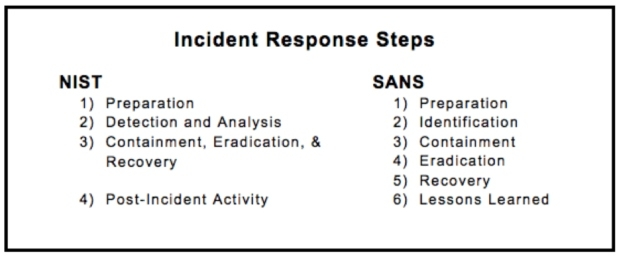
\includegraphics{./assets/img/sans-nist-ir.jpeg}

En phase de réponse notre objectif est de comprendre ce qui s'est passé sur notre système d'information grâce aux précieuses données obtenues lors de la phase de détection dans le but de trouver l'attaquant, réparer les dégâts que nous aurions subis et minimiser l'impact de son activité sur notre métier. Nous l'avons vu plus haut, une réponse à incident de manière traditionnelle se déroule en différentes étapes selon la méthodologie du SANS ou du NIST.

D'un point de vue technique, utile dans une philosophie d'automatisation, le Docteur Brian Carrier regroupe ces étapes en deux grands processus : l'investigation et l'atténuation ou \emph{mitigation}.

\subsection{L'investigation}\label{linvestigation}

Pendant l'investigation nous devons collecter et analyser les données de nos terminaux impactés par l'attaque ou susceptible d'être compromis. Nous procédons en général

\begin{enumerate}
\def\labelenumi{\roman{enumi}.}
\item
  en définissant premièrement des questions auxquelles nous n'avons pas encore des réponses
\item
  en collectant les données nécessaires pour répondre à ces questions
\item
  en analysant ces données pour y retirer de l'information intelligente
\item
  en répondant enfin à nos questions
\end{enumerate}

Concrètement nos questions seront orientées selon l'avancée de notre réponse. En début d'investigation nous allons d'abord chercher à trier les données reçues pour se focaliser sur les pistes qui nous semblent le plus pertinentes (c'est l'étape de \textbf{triaging}). Nous allons nous demander quels sont les terminaux compromis, à quel niveau sont-ils impactés, etc. ? Si notre phase de détection est optimale nous aurions déjà la réponse à certaines de ces questions.

Ensuite nous allons approfondir notre questionnement en nous demandant, qui est l'acteur présent au sein de notre système, quand a-t-il pénétré notre réseau, quels sont ses objectifs ? À ce moment nous faisons de l'analyse forensique pour corréler nos données collecter avec les actions de l'attaquant pour en extraire des informations factuelles. Cette étape nous amène à approfondir davantage le questionnement afin de trouver des preuves tangibles, comme la recherche d\textquotesingle un fichier spécifique sur une machine distante dans un état déterminé.

\subsection{L'atténuation}\label{lattuxe9nuation}

Durant l'étape d'atténuation notre souhait est de minimiser l'impact de l'attaque en cours ou subis. Cela peut être de bloquer les connexions réseaux sur les machines compromises. L'atténuation est cruciale pour empêcher l'avancée de l'attaque en plus de nous faire gagner du temps dans l'élimination de la menace. Elle devrait en principe se faire en parallèle de l'investigation, dès la détection de la menace. Cependant certaines équipes priorisent d'autres tâches de réponse par manque de ressources humaines.

Ce procédé dépend de l'attaque subie, ainsi nous n'automatiserons pas l'atténuation d'une infection par un fichier malveillant ou d'une attaque par dénis de service. Notre processus doit donc prendre en compte les éléments fournis lors de la phase de détection pour orienter les actions à mener.

Nous pouvons également ajouter sur cette optique d'automatisation le procédé de \textbf{remédiation} qui consiste à remettre en condition opérationnelle nos services. De même un processus de remédiation dépend du type d'attaque subie mais en plus elle dépend également de notre architecture et des composants compromis.

À chacune de ces étapes nous devons évaluer le niveau d'automatisation voulu comme aborder plus haut pour pouvoir ajuster nos efforts à nos besoins. Voyant à quoi cela peut ressembler pour la plupart des organisations.

\subsection{Automatisation contextuelle}\label{automatisation-contextuelle}

Toujours en se basant sur l'approche du Dr Brian Carrier, dans la majorité des organisations nous allons vouloir premièrement automatiser en totalité les étapes qui ne nécessitent pas une prise de décision humaine. En effet, nous pensons que ces personnes ont davantage tendance à classer leurs alertes, préfèrent sous-traiter les enquêtes complexes et ne disposent pas de suffisamment de ressources pour investir dans une plateforme d\textquotesingle apprentissage qui les aiderait à comprendre ce qui est habituel et comment coordonner les différentes phases de la réponse, y compris les environnements honeypot et autres.

\subsubsection{La collecte de données}\label{la-collecte-de-donnuxe9es}

L'Agence Nationale de la Sécurité de Systèmes d'Information nous propose DFIR ORC (Outil de recherche de compromission), qui nous aident à collecter les données de nos terminaux et nous facilite dans nos analyses forensiques. Ses fonctionnalités permettent aussi bien la recherche et l'extraction de preuve que l'analyse des données collectées : ``Il a été entièrement conçu afin de fonctionner dans l'écosystème Microsoft Windows de façon décentralisée et à grande échelle'' dit l'ANSSI.

\subsubsection{L'analyse de données de compromission}\label{lanalyse-de-donnuxe9es-de-compromission}

Hayabusa est un outil de réponse à incident développé par les professionnels de la sécurité de Yamato au Japon. Il permet d\textquotesingle analyser les événements Windows pour détecter les indices de compromission, d\textquotesingle examiner ces preuves et de créer une chronologie détaillée de l\textquotesingle attaque, entre autres fonctionnalités.

Ensuite, une organisation de taille moyenne souhaitera sûrement automatiser de manière partielle certaines décisions faciles à prendre et sans impacts sur la gestion de l'incident comme le choix des terminaux à analyser dans la suite de l'investigation.

\subsubsection{L'analyse de comportement anormal avec la prévention des intrusions}\label{lanalyse-de-comportement-anormal-avec-la-pruxe9vention-des-intrusions}

En laissant la machine ou des outils identifier les éléments qui leur semblent suspects. Les composants et logiciels de type IPS (Intrusion Prevention System) bloquent activement les menaces en fonction des politiques de sécurité définies. Nous avons par exemple Palo Alto Networks Threat Prevention, un IPS qui détecte et bloque les exploits de vulnérabilité et les logiciels malveillants qu'il reconnaît.

En acquérant de la maturité nous pourrons être amenés à automatiser les actions d'atténuation voire de remédiation sur les conséquences de l'attaque sur notre système d'information.

\subsubsection{La réalisation automatique des actions d'atténuation}\label{la-ruxe9alisation-automatique-des-actions-dattuxe9nuation}

Bloquer un utilisateur ou couper l'accès au réseau à un poste de travail sont des actions plutôt simples à exécuter quand nous sommes en pleine réponse à incident, se relayer sur un processus automatiser pour ces tâches connues d'avance, gâcherait du temps et des compétences que nous aurions pu investir dans de l'analyse de preuves.

\subsubsection{L'automatisation de la réponse avec les plateformes SOAR}\label{lautomatisation-de-la-ruxe9ponse-avec-les-plateformes-soar}

Dans ce contexte l'intégration entre nos différents outils au sein de notre plateforme de sécurité accroît leur capacité d'apprentissage continue en mettant régulièrement à jour leur base de connaissance sur les alertes que nous avons déjà subies. Les solutions SOAR (\emph{Security Orchestration, Automation, and Response}) aident concrètement les équipes de sécurité à gérer et à répondre aux incidents de sécurité de manière plus efficace et automatisée. Elles combinent l\textquotesingle orchestration, l\textquotesingle automatisation et la gestion des réponses aux incidents en un seul outil.

\begin{enumerate}
\def\labelenumi{\roman{enumi}.}
\item
  \textbf{Orchestration} : Intégration des différents outils de sécurité et des processus pour assurer une réponse coordonnée et cohérente aux incidents.
\item
  \textbf{Automatisation} : Exécution automatique de tâches répétitives et routinières pour réduire la charge de travail manuel et accélérer la réponse.
\item
  \textbf{Gestion des réponses} : Centralisation des informations sur les incidents, la gestion des workflows, et la documentation des actions entreprises pour une meilleure analyse post-incident.
\end{enumerate}

Nous pouvons citer Splunk SOAR, une solution de sécurité présentant des fonctionnalités de SOAR qui s'intègre parfaitement avec CyberTriage une solution d'accompagnement à l'analyse forensique qui automatise un grand nombre d'actions répétitives pour un analyste, notamment

\begin{itemize}
\item
  La collecte d'artefacts
\item
  L'identification de scénario d'attaque
\item
  La priorisation d'éléments à analyser et la recommandation d'artefacts pour une investigation approfondie
\item
  La réalisation de frises chronologiques de l'attaque
\item
  La collaboration entre différents analystes directement au sein de l'outil
\end{itemize}

Voici en somme les processus de sécurité que nous pouvons automatiser et optimiser, du cycle de développement à la réponse aux incidents. Ces standards de l'industrie nous aident à atteindre une posture idéale en matière de sécurité informatique. Toutefois l'implémentation de ces dernières doit être en adéquation avec nos besoins, notre contexte métier et notre maturité organisationnelle.

En tant qu'ingénieur sécurité en apprentissage chez Shadow et ayant développé une appétence pour l'automatisation des processus de sécurité informatique en général et les pratiques DevSecOps en particulier, mon rôle a été de mettre en place les recommandations que nous venons d'étudier. Abordons donc les étapes concrètes et les outils que j'ai utilisés dans le contexte de mise en place d'une plateforme de sécurité automatisé chez Shadow.

\begin{center}\rule{0.5\linewidth}{0.5pt}\end{center}

\chapter{Mise en place des pratiques au sein de Shadow}\label{mise-en-place-des-pratiques-au-sein-de-shadow}

Dans son contexte et dans son processus de développement, Shadow prit la décision de s'orienter vers la philosophie DevOps en mettant en place un certain nombre de procédés et d'outillages pour automatiser la mise en condition opérationnelle de ses produits et de ses outils internes.

Dans cette optique nous avons également voulu remettre la sécurité au centre de ces procédés pour nous permettre de réaliser un Shift Left avec nos processus de sécurité. Nous allons donc aborder dans cette partie les pratiques DevOps déjà en place chez Shadow avant de parler de notre plan vers le Shift Left puis nous verrons les actions et outils que j'ai mis en place pour concrétiser ce plan et nous finirons par une projection sur l'automatisation des processus de détection et de réponse.

\section{Shift Left Retro Planning}\label{shift-left-retro-planning}

Pour commencer à Shift Left, la première des choses est de réaliser une prise de conscience au sein de l'équipe sécurité d'un besoin d'évolution en ce qui concerne les pratiques de sécurité déjà en place au sein du cycle de développement. Par la suite réaliser un Shift Left implique une symbiose entre évolution culturelle, entraînement, intégration d'outils et de nouveau processus.

Pour cela, Florent, Head of Security chez Shadow, intégra dans la vision long terme de la politique de sécurité de Shadow des étapes en vue de réaliser un Shift Left au sein de nos processus. Parmi ces étapes nous pouvons retrouver :

\begin{enumerate}
\def\labelenumi{\roman{enumi}.}
\item
  la sensibilisation des collaborateurs aux problématiques de sécurité de l'organisation,
\item
  l'intégration de différents outils permettant l'automatisation de certains processus,
\item
  la mise en places de pratiques DevSecOps,
\item
  la gestion de vulnérabilité,
\item
  la modélisation des menaces auxquelles Shadow pourrait faire face.
\end{enumerate}

Certaines de ces étapes ont pu être réalisées en parallèle pendant que d'autres nécessitent une certaine maturité organisationnelle pour être débutées comme la modélisation des menaces. Cela est possible car Shadow s'est naturellement tourné vers une approche DevOps dans sa genèse. Bien qu'elles ne soient pas un prérequis pour réaliser un Shift Left, les pratiques DevOps procurent une bonne base pour procéder à ce changement tout comme l'approche DevSecOps se présente comme un fil rouge pour nous aider dans notre démarche.

\subsection{DevOps chez Shadow}\label{devops-chez-shadow}

DevOps est avant tout une approche collaborative entre les équipes de développement et les équipes opérationnelles qui se suit par un certain nombre de pratiques et d'automatisation tout au long du cycle de développement. Shadow possède dans toutes ses équipes un cycle d'intégration continue et de déploiement continu (CI/CD). Ces derniers incluent la plupart du temps une phase de linting, packaging puis de build intégré à des outils relativement modernes bien que variant d'une équipe à l'autre.

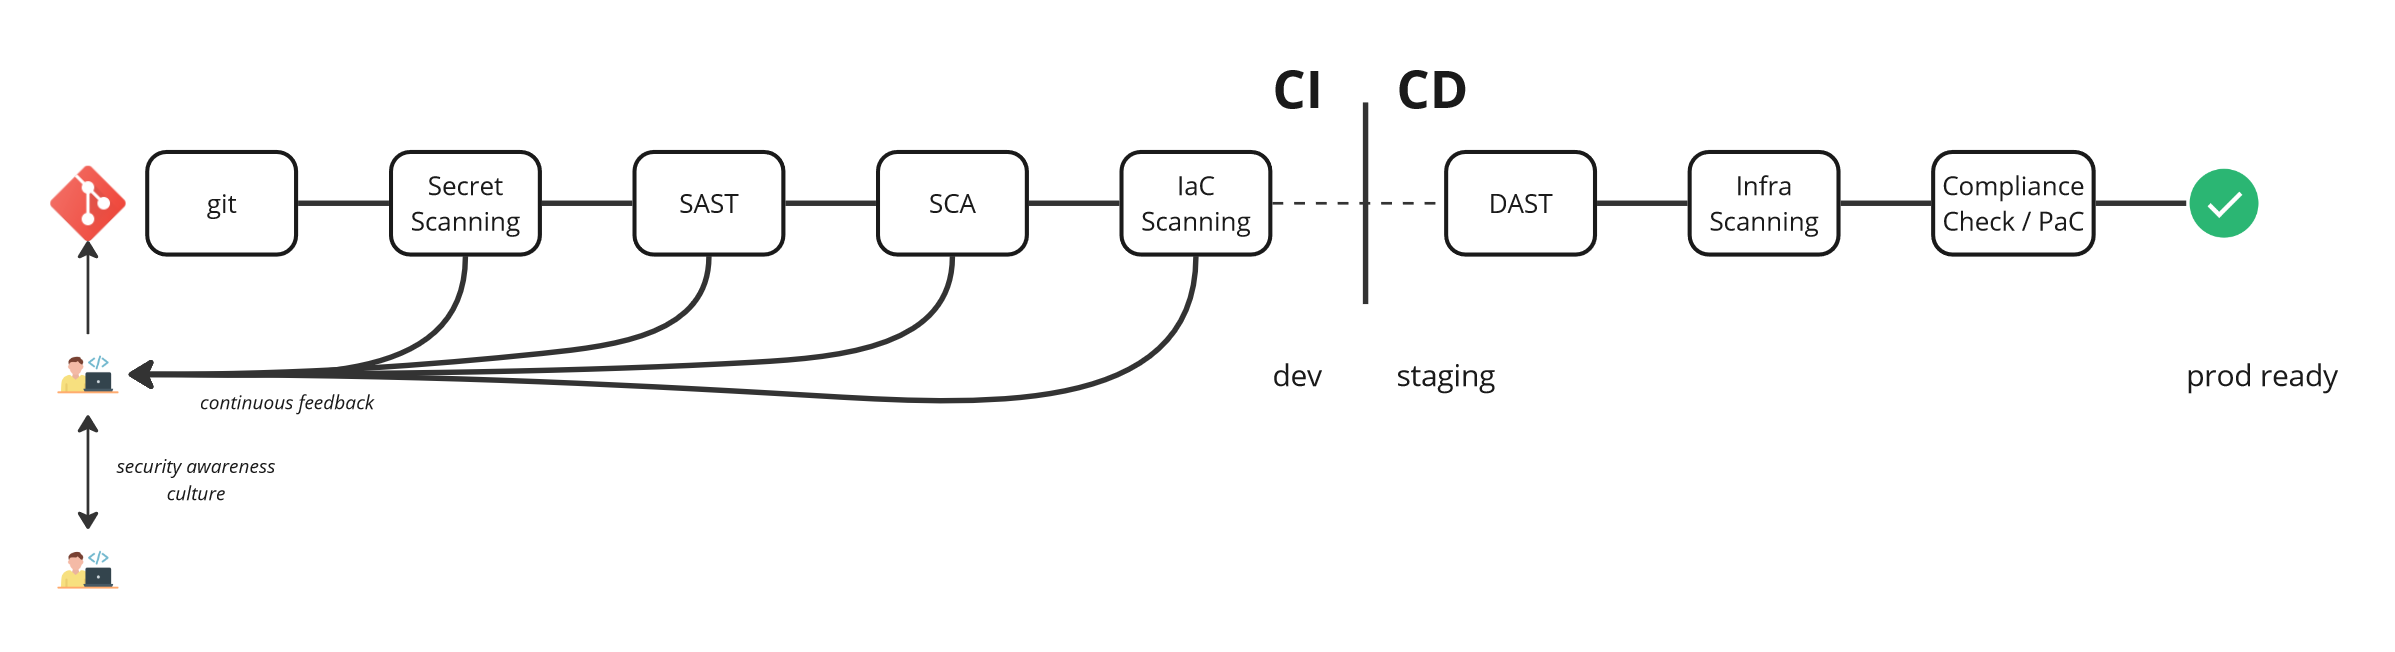
\includegraphics{./assets/img/sec_ci_cd.png} Par conséquent notre prochaine étape dans l'évolution de nos pratiques DevOps consiste à standardiser nos procédés et nos outils tout en incluant les tests de sécurité au plus tôt dans nos CI.

\section{Pratiques DevSecOps chez Shadow}\label{pratiques-devsecops-chez-shadow}

Nous avons souligné que l\textquotesingle adoption d\textquotesingle une approche DevSecOps engage tous les métiers intervenant dans le cycle de développement, en les rendant responsables de la sécurité. Cette culture est tout aussi essentielle que l\textquotesingle automatisation des processus. C\textquotesingle est pourquoi nous avons mis en place un programme de sensibilisation à la sécurité informatique à destination de nos collaborateurs.

\subsection{Programme de sensibilisation}\label{programme-de-sensibilisation}

Pour établir une culture de collaboration sur les sujets de sécurité nous devons sensibiliser nos collaborateurs aux risques de sécurité, aux bonnes pratiques et aux différents types d'attaque qui existent, notamment celle à laquelle ils sont le plus susceptibles d'être vulnérable : le phishing. En effet la majorité des organisations qui se font compromettre réussissent un accès initial grâce aux phishings car un collaborateur n'a pas été assez précautionneux dans la vérification de l'authenticité de l\textquotesingle e-mail reçu.

Mon objectif était donc de trouver une solution permettant de faire grandir les connaissances en sécurité de l'information au sein de sein de Shadow, tout en entraînant nos collègues à être alerte lors de la réception d'un e-mail paraissant suspect.

Cela nous a nécessités différentes étapes

\begin{enumerate}
\def\labelenumi{\roman{enumi}.}
\item
  Comprendre les lacunes et les besoins de renforcement en culture de sécurité informatique
\item
  Entraîner nos collaborateurs de manière régulière
\item
  Evaluer les progrès avec des exercices de simulations
\item
  Répéter cela dans une optique d'amélioration continue
\end{enumerate}

Dans une philosophie d'automatisation de processus de sécurité, nous avons compris que réaliser ces étapes manuellement avec la taille de notre équipe de sécurité serait très chronophage et perdrait continuellement de la valeur par rapport à nos occupations quotidiennes. La charge qui m'a été accordée fut de faire une analyse comparative de différentes solutions et services de sensibilisation à la sécurité informatique proposant des modules d'entraînement. Je me suis donc basé sur la liste de fonctionnalité suivante avec leur priorité pour choisir une solution correspondant à nos besoins. (Voir annexe 2)

Après avoir établi une liste de solutions open source et payantes, en priorisant les solutions européennes, car Shadow s\textquotesingle oriente vers la souveraineté numérique, j\textquotesingle ai dû évaluer chacune de ces solutions à travers des échanges commerciaux, des démonstrations et des phases de PoC (preuve de concept) sur une population donnée d\textquotesingle employés de Shadow, puis filtrer celles qui nous convenaient aussi bien fonctionnellement que financièrement. Le ressenti des futurs utilisateurs a également été pris en compte dans le choix de la solution, ce qui nous a permis d\textquotesingle obtenir une moyenne pondérée de chaque solution à l\textquotesingle aide des notes que les utilisateurs --- nos collaborateurs --- ont pu attribuer à ces solutions en se basant sur des critères préalablement définis.

J'introduis donc Riot une solution dédiée à la sensibilisation à la sécurité informatique. Elle vise à former les employés d\textquotesingle une entreprise aux bonnes pratiques en matière de sécurité informatique. Riot propose une approche ludique et engageante pour aider les utilisateurs à mieux comprendre les menaces de sécurité et à adopter les comportements appropriés pour se protéger et protéger leur organisation.

Voici quelques caractéristiques de Riot :

\begin{enumerate}
\def\labelenumi{\roman{enumi}.}
\item
  \textbf{Phishing Simulation} : Riot permet de créer des campagnes de simulation d\textquotesingle attaques de phishing pour évaluer et former les employés à reconnaître les tentatives d\textquotesingle hameçonnage.
\item
  \textbf{Formation via Albert} : La plateforme propose des modules interactifs et des quiz pour sensibiliser les utilisateurs aux risques liés à la sécurité informatique réaliser par Albert un robot qui envoie des messages de sensibilisation directement dans l\textquotesingle environnement de travail des utilisateurs, Slack pour notre cas.
\item
  \textbf{Personnalisation} : Les contenus de formation peuvent être personnalisés en fonction de nos besoins et du niveau de connaissance des utilisateurs.
\item
  \textbf{Suivi et Reporting} : Riot fournit des outils pour suivre l\textquotesingle engagement des utilisateurs et mesurer l\textquotesingle efficacité des campagnes de sensibilisation.
\item
  \textbf{Approche Ludique} : Pour rendre l\textquotesingle apprentissage plus attractif, Riot intègre des éléments de gamification, comme des scores et des classements.
\end{enumerate}

Riot est pour nous un outil complet pour renforcer notre posture en sécurité informatique en impliquant activement nos collègues dans le processus de sensibilisation. Cela favorise une culture de collaboration et d\textquotesingle échange sur les sujets de sécurité que nous souhaitons instaurer.

Parallèlement à cette sensibilisation continue, nous avons poursuivi notre programme de Shift Left en développant un outil de détection de valeurs secrètes pour nos projets internes versionnés sur GitLab

\subsection{Détection de secrets}\label{duxe9tection-de-secrets}

La détection de secrets sur les projets versionnés est l'une des premières étapes dans un processus de Shift Left. L'objectif étant de s'assurer qu'aucune information sensible ne soit retrouvée sur un dépôt git. En effet plusieurs compromissions surviennent suite à la découverte d'informations sensibles poussée sur des projets comme des clés d'API. Nous devons donc analyser nos commits à la recherche de toutes données secrètes.

L\textquotesingle approche idéale consiste à détecter et à prévenir l\textquotesingle exposition de données sensibles avant qu\textquotesingle elles n\textquotesingle atteignent le dépôt, car elles sont alors visibles dans l\textquotesingle historique. Dans le cas des plateformes d\textquotesingle hébergement de code, les secrets peuvent encore traîner sur le web et faire l\textquotesingle objet de recherches après avoir été retirés du dépôt. Une approche complémentaire consiste à analyser le dépôt à la recherche d\textquotesingle informations sensibles, puis à les supprimer ; il convient de noter que si des informations confidentielles sont divulguées, c\textquotesingle est qu\textquotesingle elles sont déjà compromises et qu\textquotesingle elles doivent être invalidées. La détection de secrets implique donc d'avoir une bonne méthodologie de gestion de secrets au sein de l'organisation. Nous utilisons la solution Vault de Hashicorp à cet effet. Elle permet de stocker les secrets de manière sécurisée, en les chiffrant avant de les sauvegarder dans une base de données. Vault fournit un système de contrôle d\textquotesingle accès rigoureux qui définit qui peut accéder à quels secrets. Les politiques d\textquotesingle accès peuvent être configurées pour permettre un contrôle granulaire. En plus de cela il est également possible de gérer la rotation des clés et de créer des automatisations avec toutes ces fonctionnalités. Chez Shadow notre plateforme de gestion de secrets est automatiquement déployée et configuré de manière déclarative en Infra as Code, réduisant d'office la charge de travail pour toutes les équipes.

De ce fait nous savons que faire lors de l'identification d'un nouveau secret.

\subsubsection{Comment détecter des secrets}\label{comment-duxe9tecter-des-secrets}

Pendant notre processus de réflexion sur la mise en place de cette pratique au sein des équipes de développement de Shadow, nous avons fait une étude sur la détection de secrets sur les dépôts git et l'endroit idéal pour le faire selon notre contexte. Il est intéressant de noter que Shadow, de son passé de start-up a gardé un long moment une philosophie delivery-first, c'est-à-dire prioriser la livraison aux détails opérationnels ou de sécurité. De ce fait chaque équipe n'est pas alignée sur un standard dans leur cycle de développement. Ainsi, dans une vision d'implémentation de bonnes pratiques et d'amélioration des processus en cours nous avons quelques contraintes organisationnelles et une once de nostalgie vis-à-vis des processus déjà en place.

Nous avons vu que la détection de secrets peut se faire

\begin{itemize}
\item
  \textbf{Localement} avant que le code ne soit versionné à l'aide de pre-commit, ce qui implique une détection préalable du secret bien que dépendant de la volonté de l'utilisateur à implémenter l'outil proposé
\item
  \textbf{Pendant l'intégration continue} (CI), un secret détecté à ce niveau serait déjà compromis, néanmoins l'équipe en charge serait la mieux placée pour juger de la pertinence du secret détecté, du processus d'invalidation et de la correction du code impliqué.
\item
  \textbf{Durant une analyse des sources après que le code ait été poussé}, cela est à la charge de l'équipe sécurité et implique une bonne gestion des secrets remontée tout en prenant en compte l'identification des faux positifs. Le défaut étant que ce procédant est non bloquant dans le cycle de développement et le processus d'invalidation, restant à la charge des équipes de développement ne serait pas nécessairement immédiat.
\end{itemize}

Cette dernière solution nous a paru être un bon compromis pour notre situation. Nous avons donc développé Gitleaker, une API de détection de secrets exposées qui agit à chaque fois qu'un nouveau code est poussé sur notre espace au sein de la plateforme GitLab et notifie l'auteur sur Slack en cas de nouveaux secrets exposés.

\subsubsection{Gitleaker}\label{gitleaker}

Gitleaker utilise \emph{gitleaks} comme outil de détection de secrets, il permet de rechercher divers types d'information sensible en se basant sur le contenu de l'historique de commits. D'autres outils existent comme

\begin{itemize}
\item
  \emph{gittyleaks} : Recherche d\textquotesingle informations sensibles pour un dépôt git un peu comme \emph{gitleaks}, cependant il est plus vieux et moins maintenu que \emph{gitleaks}.
\item
  \emph{git-secrets} : Empêche de versionner des secrets grâce à un module complémentaire qui s'intègre à la commande \emph{git.}
\end{itemize}

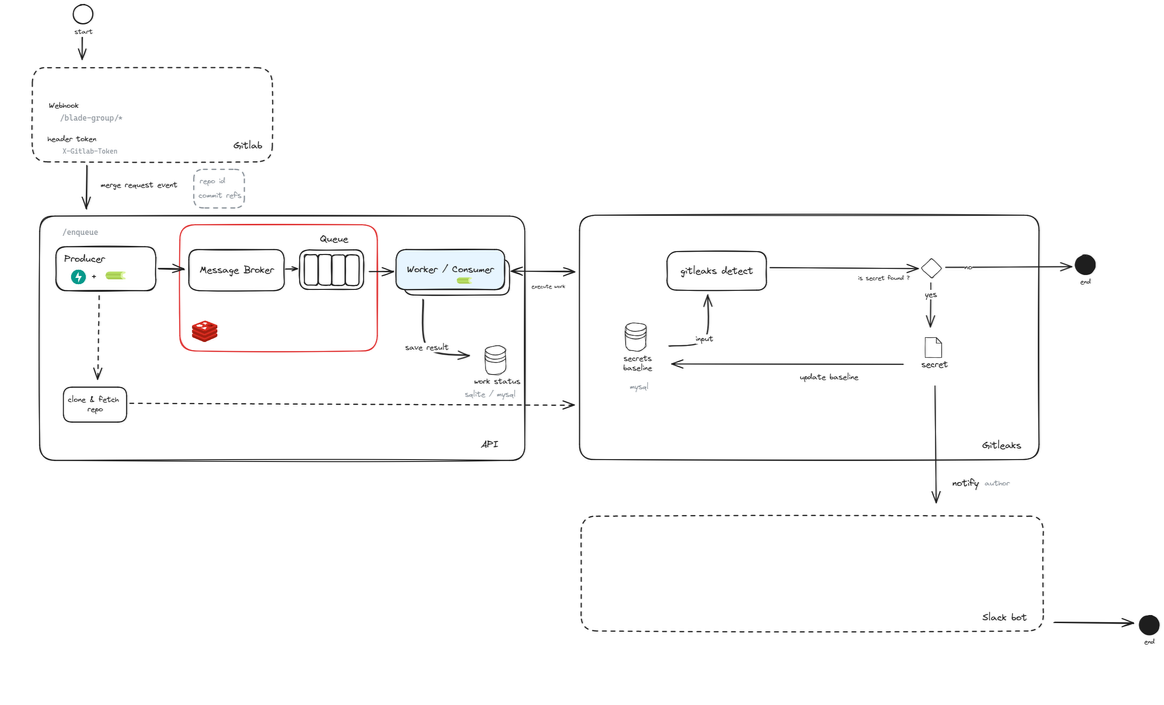
\includegraphics{./assets/img/gitleaks_webhooks_workflow.png} Voici un schéma d'architecture décrivant également le processus de traitement d'une requête

Durant le processus de développement j'ai dû prendre en compte diverses contraintes pour assurer que l'API supporte de fortes charges et soit à même d'évoluer rapidement. D'où la présence d'un modèle de file d'attente utilisant Redis et la librairie python celery. J'ai également pu éprouver le cycle d'intégration et de déploiement en continu expliqué plus haut afin de justifier l'application de nouvelles pratiques DevSecOps nous permettant d'adopter une approche de Shift Left.

La détection de secret n'est qu'une première brique dans l'exécution de tests de sécurité au sein de notre cycle d'intégration continue. La prochaine étape est d'ajouter des outils d'analyse statique et dynamique de code pour identifier les vulnérabilités qui s'y cache et d'avoir une approche de gestion de ces vulnérabilités permettant d'évaluer, atténuer ou remédier le risque d'exploitation de ces dernières. Dans cette optique nous avons identifié DefectDojo.

\subsubsection{DefectDojo}\label{defectdojo}

DefectDojo est une plateforme de gestion de vulnérabilités open source proposant des fonctionnalités d'importation de rapports d'une multitude d'outils de sécurité, de suivi d'état de la vulnérabilité --- de l'identification à la remédiation ou l'acceptation --- de déduplication avec les vulnérabilités déjà remontées et possède une API permettant de réaliser diverses intégrations et automatisation entre nos outils et les fonctionnalités offertes par la plateforme.

En vue d'intégrer cette plateforme à notre catalogue, je me suis chargé de juger la pertinence de cette dernière dans un environnement local en créant un processus automatisé dont l'objet fut d'importer les résultats d'une analyse statique de code --- utilisant Semgrep un outil d'analyse multilangage --- réalisé à chaque nouveau code poussé sur le dépôt. L'objectif étant que chaque utilisateur ayant accès à la plateforme soit responsable de l'état de la vulnérabilité identifié, l'équipe sécurité s'occupant de l'accompagnement des équipes dans la qualification et les possibilités de remédiation.

Concrètement ce processus automatisé se présente comme un ensemble de scripts bash intégré à GitLab CI, nous permettant de définir un grand nombre de flux et d'actions à réaliser suite à des événements survenant sur le dépôt. À moyen terme, nous avons l\textquotesingle intention de distribuer ce modèle pour l\textquotesingle intégrer à tous les projets de Shadow et faciliter ainsi l\textquotesingle intégration des outils d\textquotesingle analyse statique et dynamique à toutes les équipes.

Pour poursuivre avec les processus de sécurité automatisés dans notre équipe, abordons comment les phases de détection et de réponse sont planifiées chez Shadow et quels procédés j'ai pu améliorer pour amoindrir la charge de travail de l'équipe sécurité.

\section{Automatisation des processus de détection et de réponse chez Shadow}\label{automatisation-des-processus-de-duxe9tection-et-de-ruxe9ponse-chez-shadow}

\subsection{Détection}\label{duxe9tection}

En plus de la détection d'incident, chez Shadow nous avons également la détection de fraude et d'abus d'utilisation de nos services. En ce qui concerne Shadow PC, nous avons des requêtes au sein de nos différents outils qui remontent les paiements suspicieux et les comptes potentiellement abusifs, cependant le processus de vérification de ces alertes est chronophage et répétitif. Nous développons des plateformes et API internes pour réaliser certaines de ces tâches de manière automatiques. Pour Shadow Drive, j'ai eu l'honneur pendant mon projet de fin d'étude de mettre en place les premiers éléments de détections et de prévention d'intrusion sur notre infrastructure.

En effet je mentionne dans mon mémoire que

\begin{quote}
Nous avons donc vu qu'il était nécessaire de connaître avant toute chose les besoins de l'entreprise en termes de sécurité en réalisant une analyse de besoins suivie d'une analyse de risques. Puis de définir un protocole de test car il sera notre boussole lors de l'évaluation des solutions de sécurité qui s'offrent à nous. Dans notre cas, nous avons étudié les solutions éditées par OGO Security, CrowdSec et UBIKA qui sont des boîtes françaises spécialisés dans la cybersécurité. Cette étude nous a prouvé que l'agent CrowdSec était le meilleur compromis pour nous avec un rapport protection coût acceptable à l'heure actuelle. Enfin pour pérenniser la sécurité de notre infrastructure et l'efficacité de la solution choisie, nous avons jugé bon de définir un processus d'amélioration continue après avoir déployé en production ladite solution. (Olea, 2023)
\end{quote}

Depuis la mise ne place de manière industrielle de CrowdSec, nous avons commencé à être alertés des robots qui analysent internet à la recherche de vulnérabilités, à bloquer de manière automatique les comportements suspects et améliorer les capacités de la solution à ne pas notifier les faux positifs.

De plus notre équipe étudie le déploiement de Wazuh un XDR présenté plus haut sur tous les terminaux et serveurs de l'entreprise pour une surveillance optimale des événements qui s'y produisent.

En parallèle nous éprouvons également les possibilités de nos plateformes et outils à nous accompagner dans la résolution de nos incidents. Voyons donc comment nous y parvenons.

\subsection{Réponse}\label{ruxe9ponse}

Comme vu dans l'Etat de l'art, automatiser la phase de réponse à incident en interne demande une certaine maturité de ses différents processus et un rapport bénéfice, coût, probabilité et impact d'une erreur sur le processus automatisé acceptable pour l'organisation. Chez Shadow notre gestion d'incident est grandement manuelle. Nous profitons des fonctionnalités de nos outils pour nos investigations et externalisons les cas d'analyse forensique. Par exemple, CrowdSec possède un mode \textbf{replay} qui permet de rejouer un fichier de journalisation afin d'y retrouver des signes de comportement malicieux et approfondir la recherche de preuves de compromission ou d'intrusion.

Étant en cours de Shift Left, nous restons proactifs et définissons continuellement de nouvelles étapes dans notre démarche et apprenons à chaque nouveau jalon atteint dans notre planification.

\section{Amélioration continue et prochaines étapes}\label{amuxe9lioration-continue-et-prochaines-uxe9tapes}

Dans une optique d'amélioration continue de nos processus, chez Shadow et en général, une équipe de sécurité se doit de remettre ses pratiques en question pour les faire évoluer. La sécurité est un voyage, il est tout à fait normal de changer de route lorsque celle que nous suivons semble nous éloigner de notre destination.

C'est pourquoi, nous avons déjà prévu la suite de nos actions avec ce que nous avons déjà en place.

\begin{enumerate}
\def\labelenumi{\roman{enumi}.}
\item
  L'ajout au sein de nos CI/CD d'outils d'analyse dynamique.
\item
  Poursuivre avec la vérification en continue de conformité selon différents standards industriels comme SecNumCloud ou PCI DSS.
\item
  Nous avons cité plus haut la gestion de vulnérabilité semi-automatisée avec la plateforme open source DefectDojo.
\item
  La détection de comportements frauduleux dans le contexte de Shadow Drive grâce à CrowdSec notamment la création automatique de compte ou tout usage qui sortirait de nos conditions.
\item
  L'implémentation de CrowdSec au sein de toutes les équipes afin de profiter de la fonctionnalité de partage d'information entre les différentes instances de la solution.
\item
  L'affinement des processus de réponse et l'intégration de nos différents outils à une plateforme unique de gestion d'événements.
\end{enumerate}

Ces différents éléments sont une liste non exhaustive de ce que nous avons prévu de faire pour parfaire ce que nous faisons dans l'équipe sécurité tout en intégrant nos collaborateurs car nous avons un objectif commun : la satisfaction de nos utilisateurs en garantissant le maintien en condition opérationnelle de nos services.

\chapter{Conclusion}\label{conclusion}

En conclusion, à l\textquotesingle ère où l\textquotesingle agilité et la réactivité sont essentielles pour rester compétitif, il devient impératif d\textquotesingle intégrer la sécurité dès les premières phases du développement mais également faire évoluer ses processus de détection et de réponse en automatisant les tâches répétitives.

Nous nous sommes demandé en début de cette thèse professionnelle comment la mise en place des pratiques de sécurité automatisée au sein des processus de développement peut améliorer la résistance des systèmes d\textquotesingle information aux menaces qui pèsent sur une organisation et augmenter la performance des équipes de sécurité car nous avons pris conscience de la charge de travail imputé aux équipes de sécurité dans un monde où presque toutes les équipes participant au développement d'un produit prennent des décisions de sécurité impactant toute l'organisation. D'où la nécessité de faire évoluer nos pratiques dans une vision collaborative de la sécurité de l'information.

Au vu de ce qui précède, l'industrie recommande aujourd'hui d'opter pour une approche de Shift Left où nous intégrant la sécurité au plus tôt dans le cycle de développement. À cela nous ajoutons une part d'automatisation au sein des phases de détection de la menace et de réponse à incident pour redonner de la vélocité aux équipes perdant du temps dans des tâches sans grande valeur ajoutée à leur mission.

Il est cependant intéressant de noter qu'un cycle de développement sécurisé ne comble pas un manquement de sécurité physique. De plus l'automatisation des processus peut grandement nous être utile tout en ajoutant des problèmes annexes comme le maintien des outils développés, la gestion des faux positifs impliquant d'améliorer les algorithmes développés ou d'appliquer des règles plus fines ou encore l'augmentation de la surface d'attaque de l'organisation en laisser passer de nouvelles vulnérabilités. Avec l'automatisation vient également un risque de perte de compétences, il devient difficile d'apprendre à de nouvelles recrues les tâches basiques si elles sont toutes automatisées. Enfin si tout le système mis en place vient à ne plus fonctionner et que les personnes en charge ne savent plus réaliser les tâches automatisées de manière manuelle, l'automatisation devient plus une épée de Damoclès qu'une solution au manque d'efficacité de l'équipe.

En fin de compte l'automatisation des processus de sécurité et l'intégration de la sécurité au plus tôt dans le cycle de développement ne sont pas des solutions miracles mais sont des outils à utiliser de manière intelligente et sans dépendance pour que notre voyage nous semble léger.

\chapter{Bibliographie}\label{bibliographie}

Bell, L., Brunton-Spall, M., Smith, R., \& Bird, J. (2017). \emph{Agile Application Security.} O\textquotesingle Reilly Media, Inc.

LaPiedra, J. (2002). \emph{The Information Security Process.} SANS Institute.

Lietz, S. (2015, 06 01). \emph{What is DevSecOps?} Retrieved from devsecops.org: \url{https://devsecops.org}

Lietz, S. (2016, 06 05). \emph{Shifting Security to the Left.} Retrieved from devsecops.org: \url{https://www.devsecops.org/blog/2016/5/20/-security}

Olea, G. (2023). \emph{Mise en place d\textquotesingle une stratégie de sécurité pour une plateforme SaaS d'outils collaboratifs.} Reims.

RedHat. (2024, 03 19). \emph{Shift left vs.~shift right.} Retrieved from RedHat: \url{https://www.redhat.com/en/topics/devops/shift-left-vs-shift-right}

\chapter{Annexes}\label{annexes}

\section{Le cycle de développement sécurisé}\label{le-cycle-de-duxe9veloppement-suxe9curisuxe9-1}

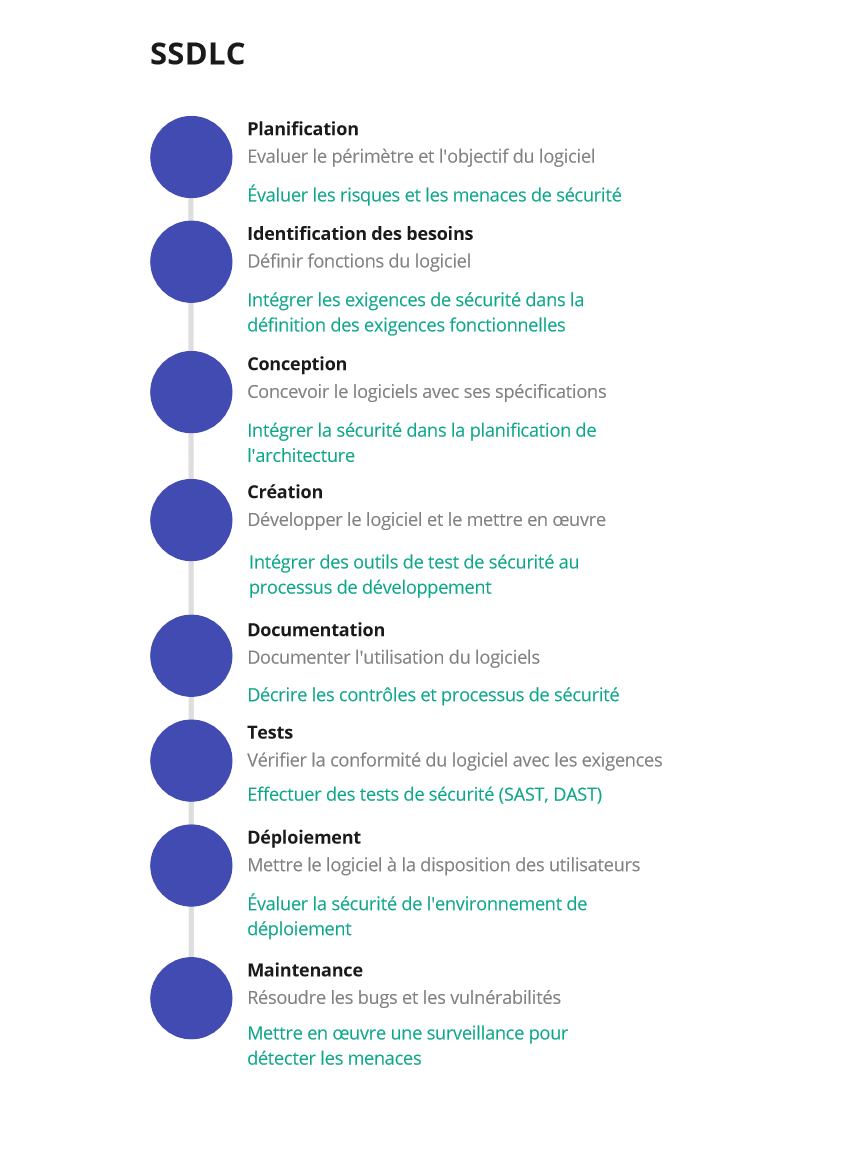
\includegraphics{./assets/img/ssdlc.png}

\section{Fonctionnalités d'une solution de sensibilisation à la sécurité}\label{fonctionnalituxe9s-dune-solution-de-sensibilisation-uxe0-la-suxe9curituxe9}

\begin{longtable}[]{@{}ll@{}}
\toprule\noalign{}
\textbf{Fonctionnalité} & \textbf{Priorité} \\
\midrule\noalign{}
\endhead
\bottomrule\noalign{}
\endlastfoot
Simulateur de campagne de phishing & 1 \\
Personnaliser le contenu & 1 \\
Catalogue de cours et de documents de formation & 1 \\
Variété de modèles & 1 \\
Intégration Slack & 1 \\
Automatiser les simulations de phishing & 2 \\
Rapports d\textquotesingle analyse & 2 \\
Attribution de contenu dynamique & 2 \\
Suivi de l\textquotesingle apprentissage & 2 \\
Gamification de la sensibilisation & 2 \\
Interface Web & 2 \\
Facile à utiliser & 2 \\
Simulation de pièces jointes à des courriels & 3 \\
Évaluation du risque sur le point de défaillance de l\textquotesingle employé & 3 \\
Possibilité pour l\textquotesingle utilisateur de signaler un courriel & 3 \\
Interface graphique & 4 \\
IA / Holistique & 4 \\
\end{longtable}

{[}{]}Tableau 1 Tableau de priorisation des fonctionnalités d\textquotesingle une solution de sensibilisation à la sécurité

  \bibliography{bib/book.bib}

\printindex

\end{document}
